\documentclass[]{article}
\usepackage{lmodern}
\usepackage{amssymb,amsmath}
\usepackage{ifxetex,ifluatex}
\usepackage{fixltx2e} % provides \textsubscript
\ifnum 0\ifxetex 1\fi\ifluatex 1\fi=0 % if pdftex
  \usepackage[T1]{fontenc}
  \usepackage[utf8]{inputenc}
\else % if luatex or xelatex
  \ifxetex
    \usepackage{mathspec}
  \else
    \usepackage{fontspec}
  \fi
  \defaultfontfeatures{Ligatures=TeX,Scale=MatchLowercase}
\fi
% use upquote if available, for straight quotes in verbatim environments
\IfFileExists{upquote.sty}{\usepackage{upquote}}{}
% use microtype if available
\IfFileExists{microtype.sty}{%
\usepackage{microtype}
\UseMicrotypeSet[protrusion]{basicmath} % disable protrusion for tt fonts
}{}
\usepackage[margin=1in]{geometry}
\usepackage{hyperref}
\hypersetup{unicode=true,
            pdftitle={Permutation Tests},
            pdfborder={0 0 0},
            breaklinks=true}
\urlstyle{same}  % don't use monospace font for urls
\usepackage{color}
\usepackage{fancyvrb}
\newcommand{\VerbBar}{|}
\newcommand{\VERB}{\Verb[commandchars=\\\{\}]}
\DefineVerbatimEnvironment{Highlighting}{Verbatim}{commandchars=\\\{\}}
% Add ',fontsize=\small' for more characters per line
\usepackage{framed}
\definecolor{shadecolor}{RGB}{248,248,248}
\newenvironment{Shaded}{\begin{snugshade}}{\end{snugshade}}
\newcommand{\KeywordTok}[1]{\textcolor[rgb]{0.13,0.29,0.53}{\textbf{#1}}}
\newcommand{\DataTypeTok}[1]{\textcolor[rgb]{0.13,0.29,0.53}{#1}}
\newcommand{\DecValTok}[1]{\textcolor[rgb]{0.00,0.00,0.81}{#1}}
\newcommand{\BaseNTok}[1]{\textcolor[rgb]{0.00,0.00,0.81}{#1}}
\newcommand{\FloatTok}[1]{\textcolor[rgb]{0.00,0.00,0.81}{#1}}
\newcommand{\ConstantTok}[1]{\textcolor[rgb]{0.00,0.00,0.00}{#1}}
\newcommand{\CharTok}[1]{\textcolor[rgb]{0.31,0.60,0.02}{#1}}
\newcommand{\SpecialCharTok}[1]{\textcolor[rgb]{0.00,0.00,0.00}{#1}}
\newcommand{\StringTok}[1]{\textcolor[rgb]{0.31,0.60,0.02}{#1}}
\newcommand{\VerbatimStringTok}[1]{\textcolor[rgb]{0.31,0.60,0.02}{#1}}
\newcommand{\SpecialStringTok}[1]{\textcolor[rgb]{0.31,0.60,0.02}{#1}}
\newcommand{\ImportTok}[1]{#1}
\newcommand{\CommentTok}[1]{\textcolor[rgb]{0.56,0.35,0.01}{\textit{#1}}}
\newcommand{\DocumentationTok}[1]{\textcolor[rgb]{0.56,0.35,0.01}{\textbf{\textit{#1}}}}
\newcommand{\AnnotationTok}[1]{\textcolor[rgb]{0.56,0.35,0.01}{\textbf{\textit{#1}}}}
\newcommand{\CommentVarTok}[1]{\textcolor[rgb]{0.56,0.35,0.01}{\textbf{\textit{#1}}}}
\newcommand{\OtherTok}[1]{\textcolor[rgb]{0.56,0.35,0.01}{#1}}
\newcommand{\FunctionTok}[1]{\textcolor[rgb]{0.00,0.00,0.00}{#1}}
\newcommand{\VariableTok}[1]{\textcolor[rgb]{0.00,0.00,0.00}{#1}}
\newcommand{\ControlFlowTok}[1]{\textcolor[rgb]{0.13,0.29,0.53}{\textbf{#1}}}
\newcommand{\OperatorTok}[1]{\textcolor[rgb]{0.81,0.36,0.00}{\textbf{#1}}}
\newcommand{\BuiltInTok}[1]{#1}
\newcommand{\ExtensionTok}[1]{#1}
\newcommand{\PreprocessorTok}[1]{\textcolor[rgb]{0.56,0.35,0.01}{\textit{#1}}}
\newcommand{\AttributeTok}[1]{\textcolor[rgb]{0.77,0.63,0.00}{#1}}
\newcommand{\RegionMarkerTok}[1]{#1}
\newcommand{\InformationTok}[1]{\textcolor[rgb]{0.56,0.35,0.01}{\textbf{\textit{#1}}}}
\newcommand{\WarningTok}[1]{\textcolor[rgb]{0.56,0.35,0.01}{\textbf{\textit{#1}}}}
\newcommand{\AlertTok}[1]{\textcolor[rgb]{0.94,0.16,0.16}{#1}}
\newcommand{\ErrorTok}[1]{\textcolor[rgb]{0.64,0.00,0.00}{\textbf{#1}}}
\newcommand{\NormalTok}[1]{#1}
\usepackage{graphicx,grffile}
\makeatletter
\def\maxwidth{\ifdim\Gin@nat@width>\linewidth\linewidth\else\Gin@nat@width\fi}
\def\maxheight{\ifdim\Gin@nat@height>\textheight\textheight\else\Gin@nat@height\fi}
\makeatother
% Scale images if necessary, so that they will not overflow the page
% margins by default, and it is still possible to overwrite the defaults
% using explicit options in \includegraphics[width, height, ...]{}
\setkeys{Gin}{width=\maxwidth,height=\maxheight,keepaspectratio}
\IfFileExists{parskip.sty}{%
\usepackage{parskip}
}{% else
\setlength{\parindent}{0pt}
\setlength{\parskip}{6pt plus 2pt minus 1pt}
}
\setlength{\emergencystretch}{3em}  % prevent overfull lines
\providecommand{\tightlist}{%
  \setlength{\itemsep}{0pt}\setlength{\parskip}{0pt}}
\setcounter{secnumdepth}{0}
% Redefines (sub)paragraphs to behave more like sections
\ifx\paragraph\undefined\else
\let\oldparagraph\paragraph
\renewcommand{\paragraph}[1]{\oldparagraph{#1}\mbox{}}
\fi
\ifx\subparagraph\undefined\else
\let\oldsubparagraph\subparagraph
\renewcommand{\subparagraph}[1]{\oldsubparagraph{#1}\mbox{}}
\fi

%%% Use protect on footnotes to avoid problems with footnotes in titles
\let\rmarkdownfootnote\footnote%
\def\footnote{\protect\rmarkdownfootnote}

%%% Change title format to be more compact
\usepackage{titling}

% Create subtitle command for use in maketitle
\newcommand{\subtitle}[1]{
  \posttitle{
    \begin{center}\large#1\end{center}
    }
}

\setlength{\droptitle}{-2em}

  \title{Permutation Tests}
    \pretitle{\vspace{\droptitle}\centering\huge}
  \posttitle{\par}
    \author{}
    \preauthor{}\postauthor{}
    \date{}
    \predate{}\postdate{}
  

\begin{document}
\maketitle

\def\simiid{\stackrel{{\mbox{\text{\tiny i.i.d.}}}}{\sim}}

\subsection{Context}\label{context}

\begin{itemize}
\tightlist
\item
  So far, all of our tests have been in a setting where:

  \begin{itemize}
  \tightlist
  \item
    we have identified a statistical model we are confident is correct
  \item
    we had a test statistic whose sampling distribution under \(H_0\) we
    could obtain either

    \begin{itemize}
    \tightlist
    \item
      analytically
    \item
      via a large-sample approximation
    \end{itemize}
  \end{itemize}
\item
  What if we are not confident we have a good statistical model, or we
  can't derive the sampling disribution of our statistic, and our sample
  size is small?

  \begin{itemize}
  \tightlist
  \item
    Use computational/sampling approaches to approximate the sampling
    distribution.
  \item
    Many variations on this idea; here we will discuss permutation tests
    for paired data.
  \end{itemize}
\end{itemize}

\subsection{Example}\label{example}

It is sometimes claimed that logging can help forests recover more
quickly after forest fires. Is there evidence for this claim?

Here's a quote from the Statistical Sleuth (Ramsey and Schafer, 2013)
describing our data:

\begin{quote}
The 2002 Biscuit Fire in southwest Oregon provided a test case.
Researchers selected 16 fire-affected plots in 2014 -- before any
logging was done -- and counted tree seedlings along a randomly located
transect pattern in each plot. They returned in 2005, after nine of the
plots had been logged, and counted the tree seedlings along the same
transects. ( Data from D.C. Donato et al., 2006. ``Post-Wildfire Logging
Hinders Regeneration and Increases Fire Risk,'' \emph{Science}, 311:
352.) The numbers of seedlings in the logged (L) and unlogged (U) plots
are {[}loaded in the R code below{]}.
\end{quote}

\begin{Shaded}
\begin{Highlighting}[]
\NormalTok{logging <-}\StringTok{ }\KeywordTok{read_csv}\NormalTok{(}\StringTok{"http://www.evanlray.com/data/sleuth3/ex0429_logging.csv"}\NormalTok{)}

\KeywordTok{ggplot}\NormalTok{(}\DataTypeTok{data =}\NormalTok{ logging, }\DataTypeTok{mapping =} \KeywordTok{aes}\NormalTok{(}\DataTypeTok{x =}\NormalTok{ PercentLost)) }\OperatorTok{+}
\StringTok{  }\KeywordTok{geom_histogram}\NormalTok{() }\OperatorTok{+}
\StringTok{  }\KeywordTok{facet_wrap}\NormalTok{(}\KeywordTok{vars}\NormalTok{(Action), }\DataTypeTok{ncol =} \DecValTok{1}\NormalTok{)}
\end{Highlighting}
\end{Shaded}

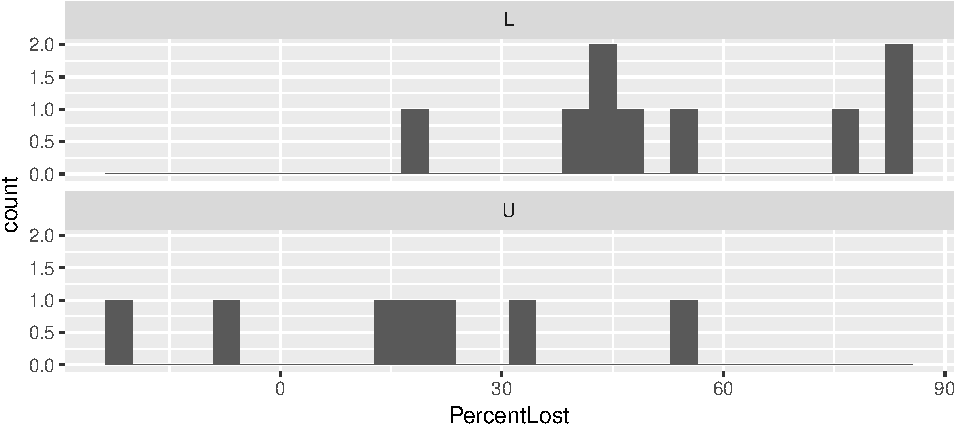
\includegraphics{20180422_permutation_test_setup_files/figure-latex/unnamed-chunk-1-1.pdf}

Let \(\mu_1\) = mean percent lost in ``population'' of plots that are
logged.

Let \(\mu_2\) = mean percent lost in ``population'' of plots that are
unlogged.

Test

\(H_0: \mu_1 = \mu_2\) vs \(H_A: \mu_1 \neq \mu_2\)

\paragraph{Option 1: Likelihood Ratio Test based on parametric
model}\label{option-1-likelihood-ratio-test-based-on-parametric-model}

\begin{itemize}
\item
  If we assume that \(X_{1i} \simiid \text{Normal}(\mu_1, \sigma^2)\)
  and \(X_{2i} \simiid \text{Normal}(\mu_2, \sigma^2)\), we can derive a
  likelihood ratio test based on t distributions.
\item
  If we don't trust that the data are normally distributed, this is
  risky (we have seen that t-based methods can fail with moderate sample
  sizes if conditions are not met).
\end{itemize}

\paragraph{\texorpdfstring{Option 2: Large-sample \(\chi^2\)
approximation to sampling distribution of likelihood
ratio}{Option 2: Large-sample \textbackslash{}chi\^{}2 approximation to sampling distribution of likelihood ratio}}\label{option-2-large-sample-chi2-approximation-to-sampling-distribution-of-likelihood-ratio}

\begin{itemize}
\tightlist
\item
  15 is not large, this is a worse idea than \#1
\end{itemize}

\paragraph{Option 3: Permutation test}\label{option-3-permutation-test}

\begin{itemize}
\tightlist
\item
  Easier to motivate with a slight modification to the hypotheses:
\end{itemize}

\(H_0\): The distributions of percent lost are the same whether or not
logging is done. (In particular, \(\mu_1 = \mu_2\))

\(H_A\): The distributions of percent lost are different depending on
whether or not logging is done. (In particular, \(\mu_1 \neq \mu_2\))

\begin{itemize}
\item
  Our test statistic will be the difference in means:
  \(W = \bar{X}_1 - \bar{X}_2\).
\item
  To calculate a p-value, we need an estimate of the sampling
  distribution of \(W\) under the condition that \(H_0\) is true.
\item
  Key ideas:

  \begin{itemize}
  \tightlist
  \item
    If \(H_0\) is true, the observed percent lost for our plots would
    have been equally likely to be observed in either the logged or
    unlogged plots.
  \item
    We will simulate many data sets that might have been observed if
    \(H_0\) was true by permuting assignments of percent lost to
    different plots.
  \end{itemize}
\end{itemize}

\begin{enumerate}
\def\labelenumi{\arabic{enumi}.}
\tightlist
\item
  Allocate storage space for difference in group means from \(nsims\)
  different samples
\item
  For \(i = 1, \ldots, nsims\):

  \begin{enumerate}
  \def\labelenumii{\alph{enumii}.}
  \tightlist
  \item
    Permute the assignments of observed values to groups
  \item
    Calculate the difference in group means, save in allocated space
  \end{enumerate}
\item
  Calculate \emph{approximate} p-value as proportion of simulated
  samples with a difference in group means at least as large as our
  observed difference in group means
\end{enumerate}


\end{document}
